\documentclass{article}

\usepackage{fancyhdr}
\usepackage[includeheadfoot,left=1in, right=0.5in, top=0.5in, bottom=0.5in]{geometry}
\usepackage{lastpage}
\usepackage{extramarks}
\usepackage[usenames,dvipsnames]{color}
\usepackage{graphicx}
\usepackage{listings}
\usepackage{courier}
\usepackage{tikz}
\usepackage{color}
\usepackage{float}
\usepackage{url}
\usepackage{subfigure}
\usepackage{varwidth}
\usepackage{caption}
\usepackage{multirow}
\usepackage[pdfborder={0 0 0}]{hyperref}
\usepackage[compact,small]{titlesec}
\usepackage{microtype}
\usepackage{verbatim}
\usepackage{booktabs}
\usepackage{indentfirst}

\parskip = 0.5\baselineskip
\setlength{\belowcaptionskip}{-\baselineskip}

\captionsetup{font=scriptsize}
\captionsetup{labelfont=bf}

\pagestyle{fancy}
\rhead{Max Thrun}
\lhead{EECE6080 - HW 4}
\rfoot{Page\ \thepage\ of \protect\pageref{LastPage}}
\cfoot{}
\renewcommand\headrulewidth{0.4pt}
\renewcommand\footrulewidth{0.4pt}

% make verbatim text small
\makeatletter
\g@addto@macro\@verbatim\small
\makeatother

\setlength\parindent{0pt} % Removes all indentation from paragraphs

\definecolor{sh_comment}{rgb}{0.12, 0.38, 0.18 } %adjusted, in Eclipse: {0.25, 0.42, 0.30 } = #3F6A4D
\definecolor{sh_keyword}{rgb}{0.37, 0.08, 0.25}  % #5F1441
\definecolor{sh_string}{rgb}{0.06, 0.10, 0.98} % #101AF9

\lstset{
    language=vhdl,
    xleftmargin=.25in,
    xrightmargin=.25in,
    numbers=left,
    numberstyle=\tiny,
    frame=tb,
    showstringspaces=false,
    captionpos=b,
    stringstyle=\color{sh_string},
    keywordstyle = \color{sh_keyword}\bfseries,
    commentstyle=\color{sh_comment}\itshape,
    basicstyle=\small\sffamily,
    %numbersep=-5pt,
    belowskip=\baselineskip,
    aboveskip=\baselineskip
}

\title{
    \vspace{2in}
    \textmd{\textbf{EECE6080 - HW 4}}\\
    \vspace{4in}
}
\author{\textbf{Max Thrun}}

\begin{document}
\maketitle

\newpage
\section*{Background \& Design}

The purpose of this lab was to implement a carry chain usuable for for an n-bit
adder. A diagram illustating the relationship between the carry chain and the
adders is shown below.

\begin{figure}[H]
    \centering
    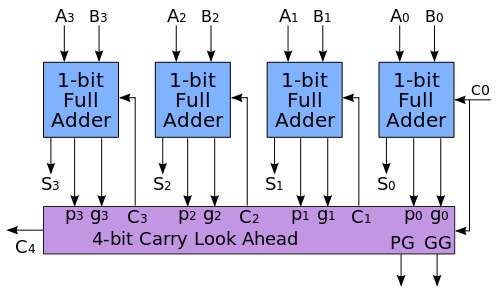
\includegraphics[width=0.8\linewidth]{../4-bit_carry_lookahead_adder.png}
    \caption{Carry Chain Design}
\end{figure}

An example of a 4-bit configuration where the carry chain is broken up into
slices is shown below.

\begin{figure}[H]
    \centering
    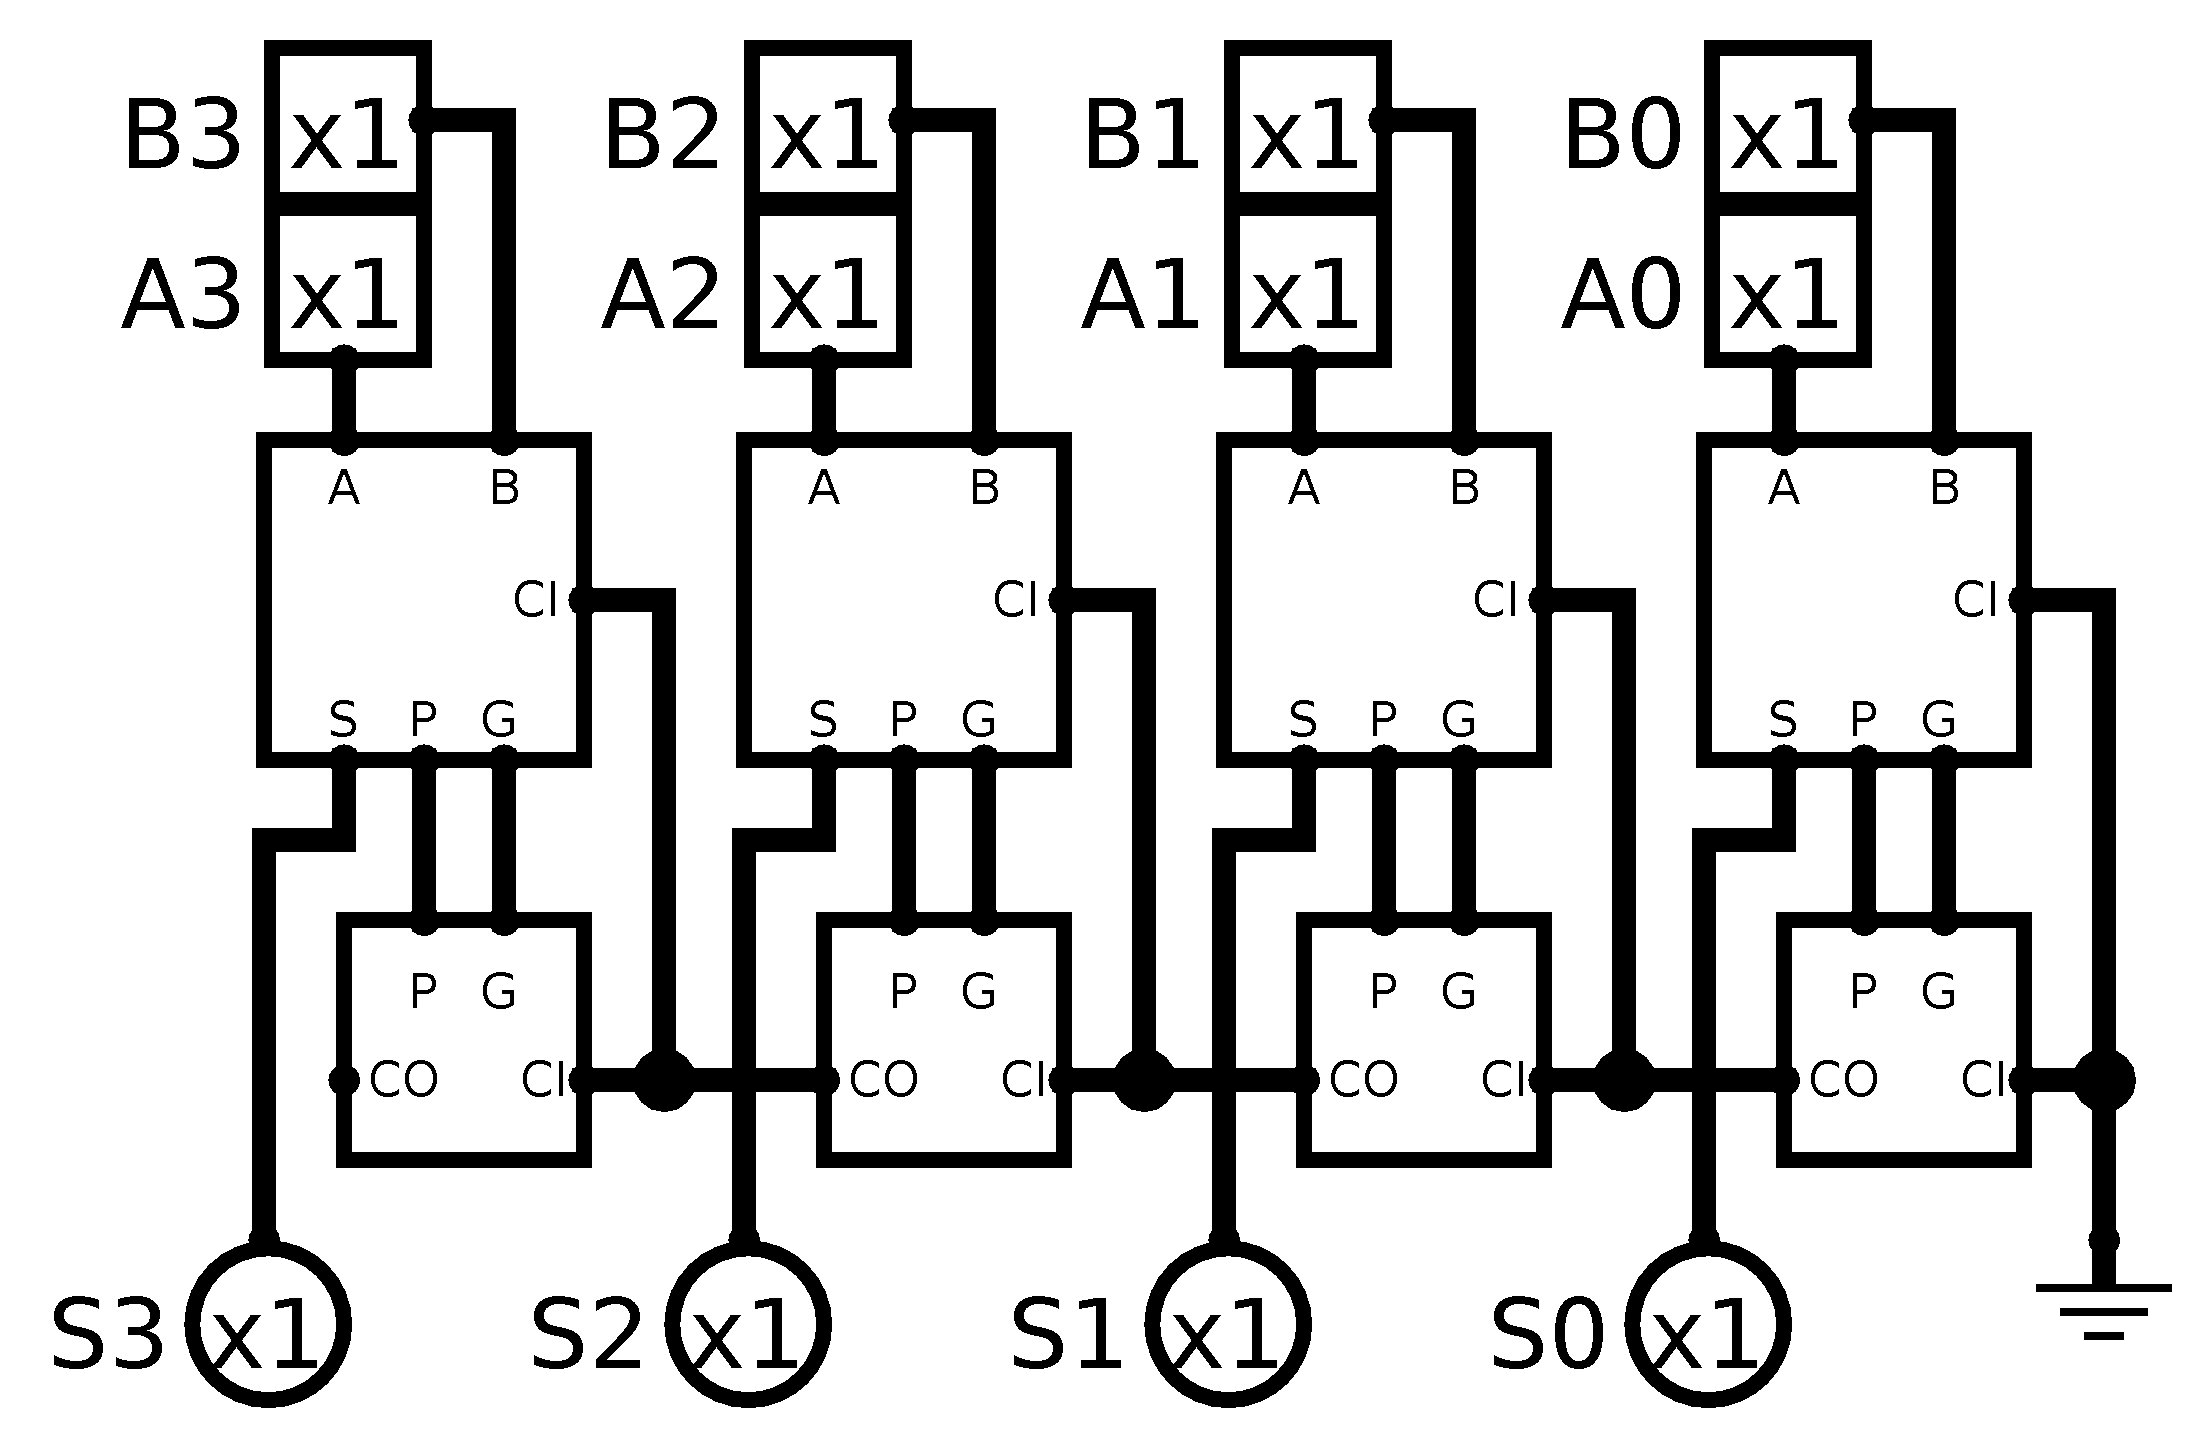
\includegraphics[width=0.8\linewidth]{../logisim_top.png}
    \caption{Top Level Design}
\end{figure}

\newpage
The logic diagram for a single carry slice using only NAND gates and static
inverters is shown below.

\begin{figure}[H]
    \centering
    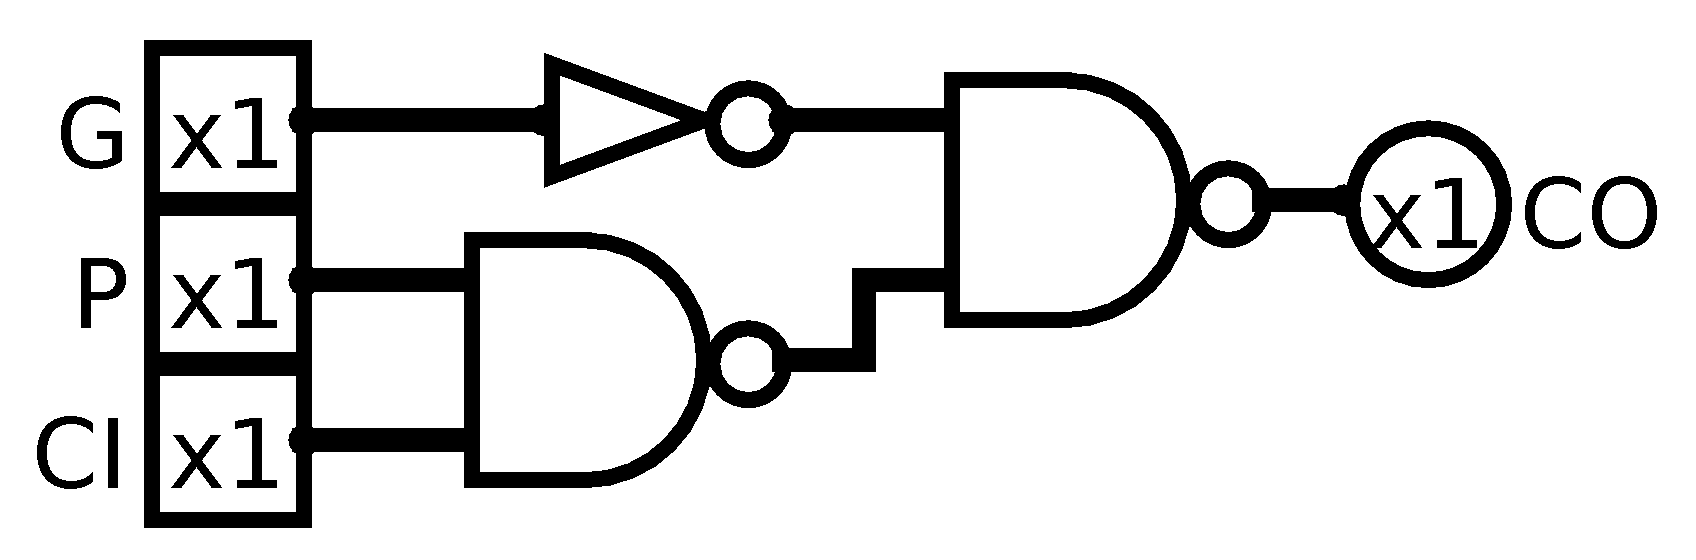
\includegraphics[width=0.8\linewidth]{../logisim_carry_slice.png}
    \caption{1-Bit Carry Design}
\end{figure}

Translating the design into a dynamic NP zipper we achieve the schematic shown below

\begin{figure}[H]
    \centering
    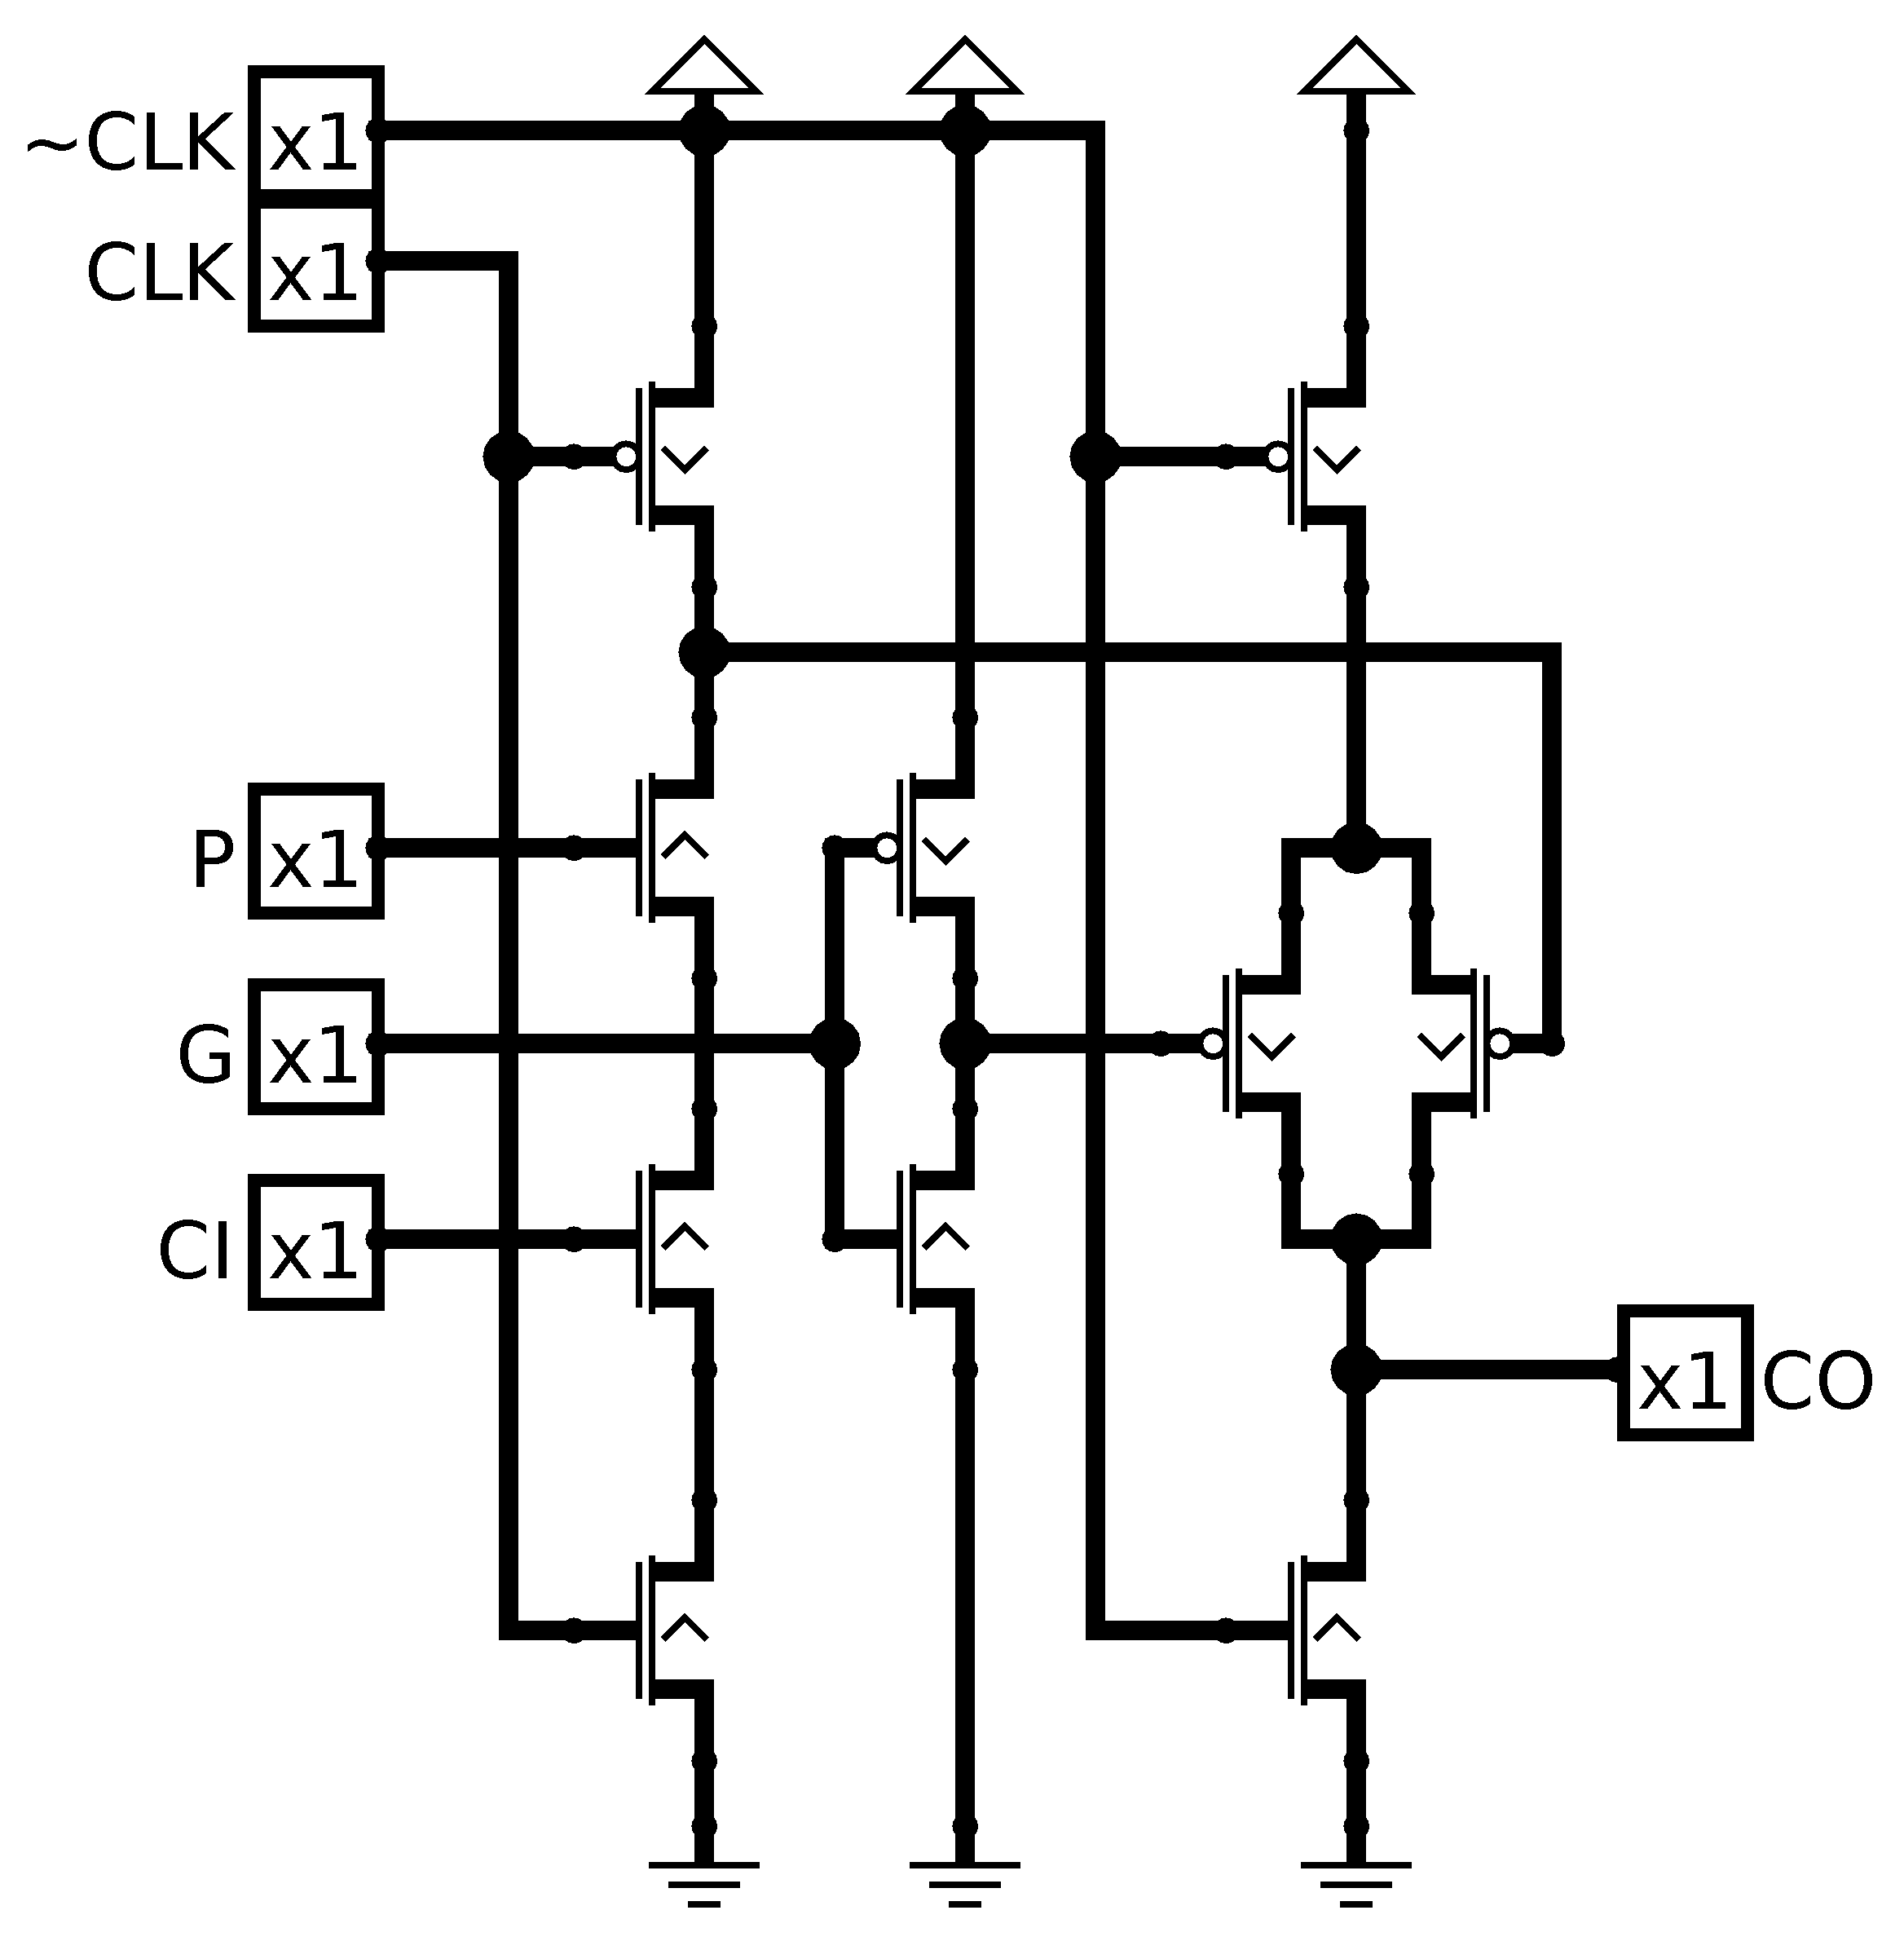
\includegraphics[width=0.8\linewidth]{../logisim_carry_slice_fets.png}
    \caption{1-Bit Carry Design Dynamic CMOS}
\end{figure}

\newpage
\section*{Part 1}

A library was created which housed subcircuits for each of the various
components used to construct the carry chain. The relevant lines for Part 1 are
shown below below.

\lstinputlisting[caption=Library,firstline=1,lastline=29]{../../models/library.sp}
\vspace{-\baselineskip}
Using the library it was trivial to instantiate and test each component of my design.
\lstinputlisting[caption=P NAND]{../part_1_p_nand.sp}
\lstinputlisting[caption=N NAND]{../part_1_n_nand.sp}
\lstinputlisting[caption=Inverter]{../part_1_inv.sp}

\newpage
The result of the P NAND simulation is shown below. It is clocked at a low
clock speed (200MHz) to ensure a full 0-5V swing on the output. From this
simulation we can measure the 10-90\% rise and fall times and use this to
estimate the max clock speed.

\begin{figure}[H]
    \centering
    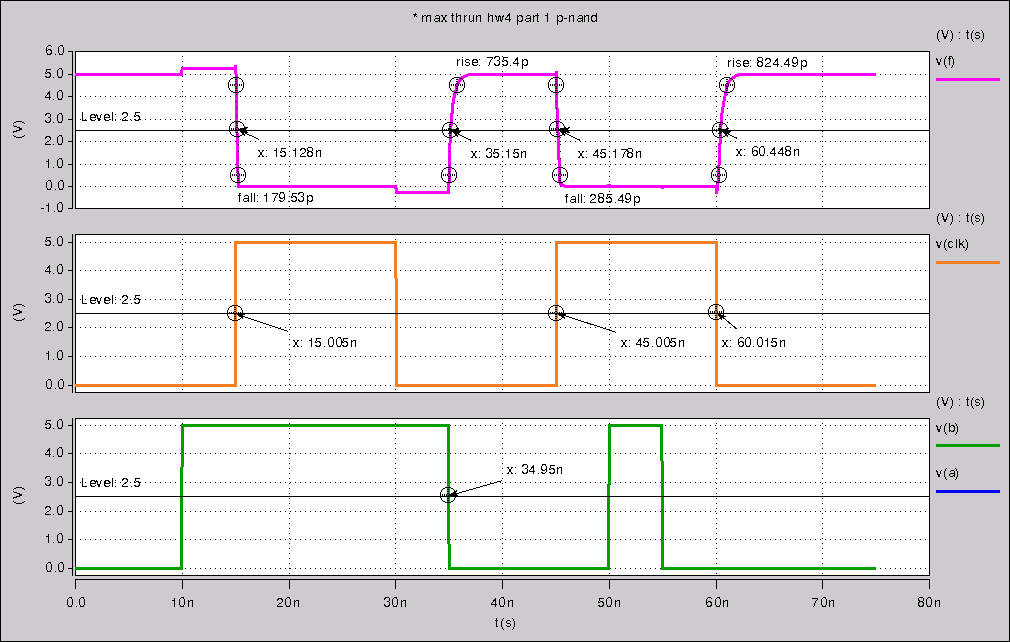
\includegraphics[width=0.8\linewidth]{../part_1_p_nand.png}
    \caption{P NAND Simulation Result}
\end{figure}

The clock speed was then increased until the output dipped below 4.5V (90\% of
5V).  The max speed of the P NAND was found to be about \textbf{530MHz}.

\begin{figure}[H]
    \centering
    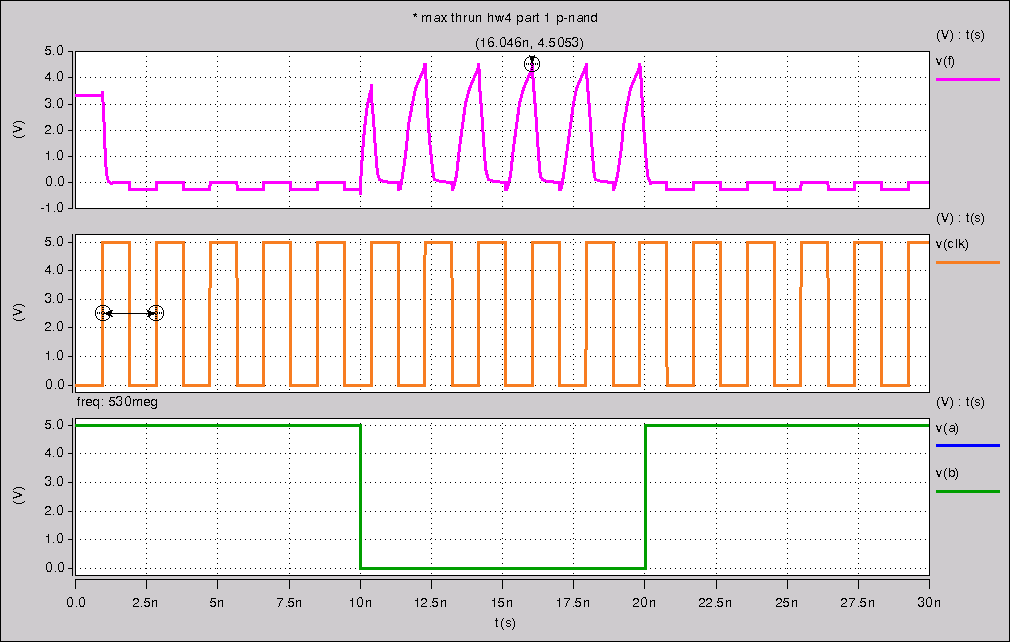
\includegraphics[width=0.8\linewidth]{../part_1_p_nand_fast.png}
    \caption{P NAND Simulation Result (Max Clock)}
\end{figure}

\newpage
The result of the N NAND simulation is shown below. Again, it was
initially clocked at a lower clock speed (200MHz) in order to mesaure the
rise and fall of the full 0-5V swing.

\begin{figure}[H]
    \centering
    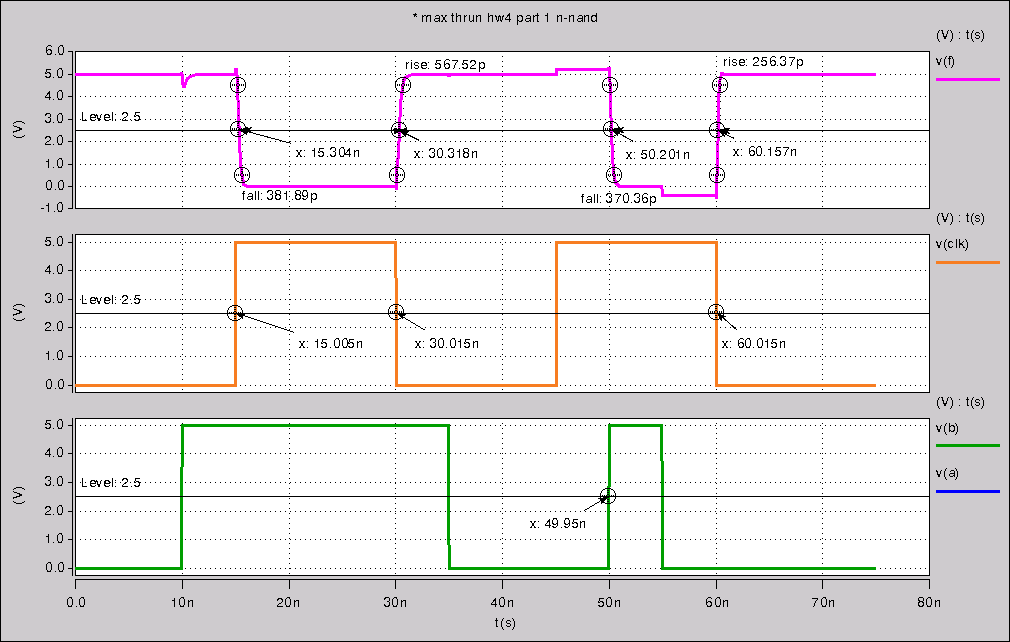
\includegraphics[width=0.8\linewidth]{../part_1_n_nand.png}
    \caption{N NAND Simulation Result}
\end{figure}

The clock speed was then increased until the output dipped below 4.5V (90\% of
5V). The max speed of the N NAND was found to be \textbf{940MHz}.

\begin{figure}[H]
    \centering
    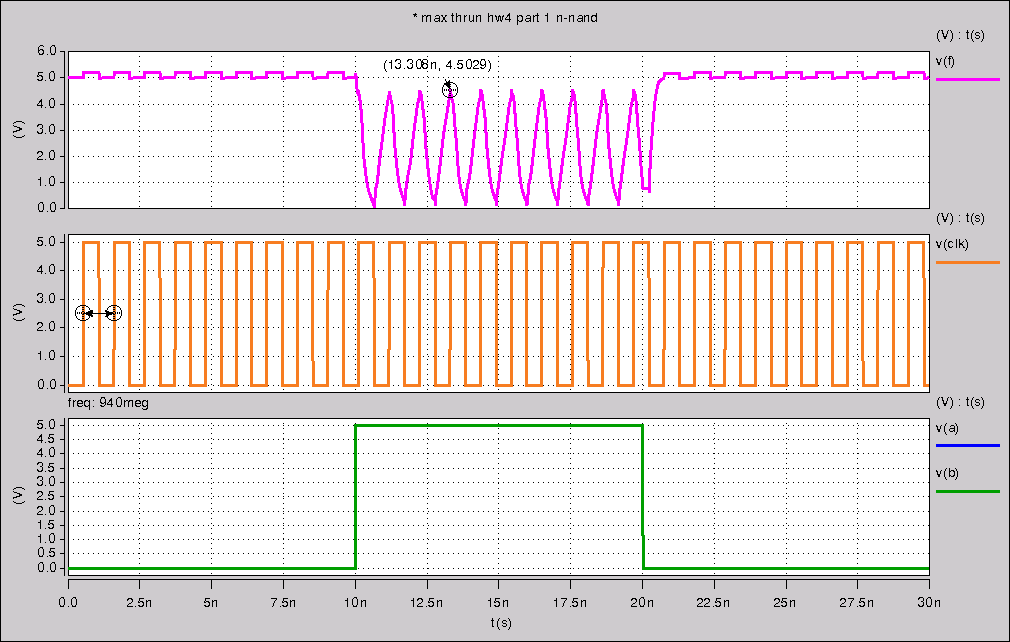
\includegraphics[width=0.8\linewidth]{../part_1_n_nand_fast.png}
    \caption{N NAND Simulation Result (Max Clock)}
\end{figure}

\newpage
A simulation of the static inverter was also done the results of which are shown below.

\begin{figure}[H]
    \centering
    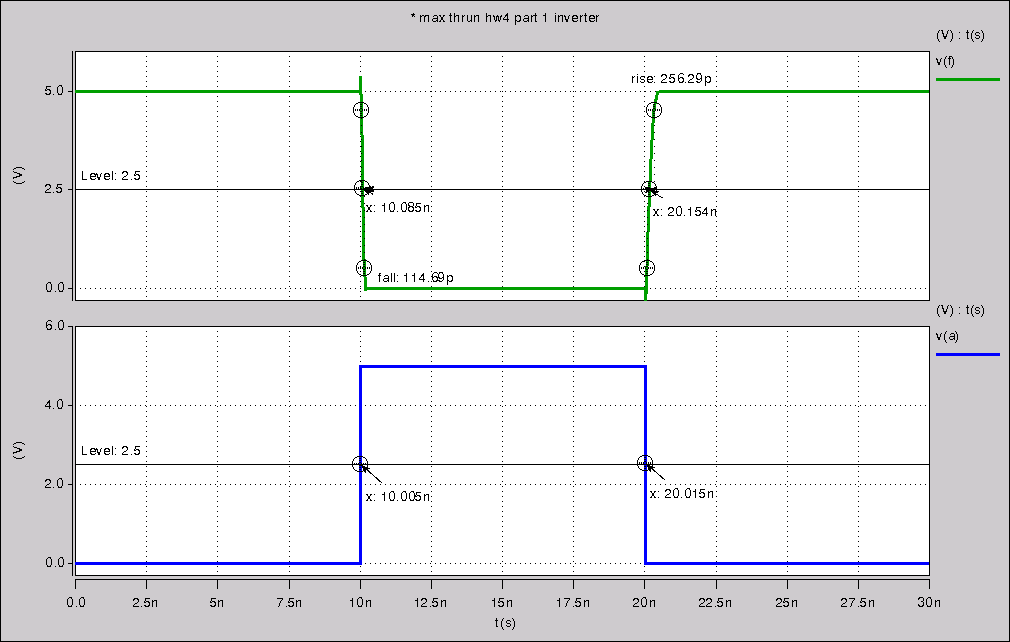
\includegraphics[width=\linewidth]{../part_1_inv.png}
    \caption{Inverter Simulation Result}
\end{figure}

\subsection*{Timing Summary}

\begin{table}[H]
    \centering
    \begin{tabular}{clll}
        \toprule
        \textbf{Component} & \textbf{Rise Time} & \textbf{Fall Time} & \textbf{Max Clock Speed} \\
        \midrule
        P NAND & 829.91p & 284.02p & 530MHz \\
        N NAND &  565.57p & 364.07p & 940MHz \\
      Inverter & 256.14p & 114.73p & 2.7GHz (calculated) \\
        \bottomrule
    \end{tabular}
    \caption{Gate Timing Summary}
\end{table}

\newpage
\section*{Part 2}

A subcircuit was added to the library which instantiates and connects the
components needed to construct a carry slice.

\lstinputlisting[caption=Library,firstline=30]{../../models/library.sp}

The carry slice was then instantiated and run through a simulation which
exercises the worst case inputs. For our carry slice the worst case condition
is when P is held at 5V, G is held at 0V. A change to CI in the condition
directly changes CO.

\lstinputlisting[caption=Part 2 Spice File]{../part_2.sp}

\newpage
The simulation was first run with a slow clock of 125MHz in order to measure
the full rise and fall time.

\begin{figure}[H]
    \centering
    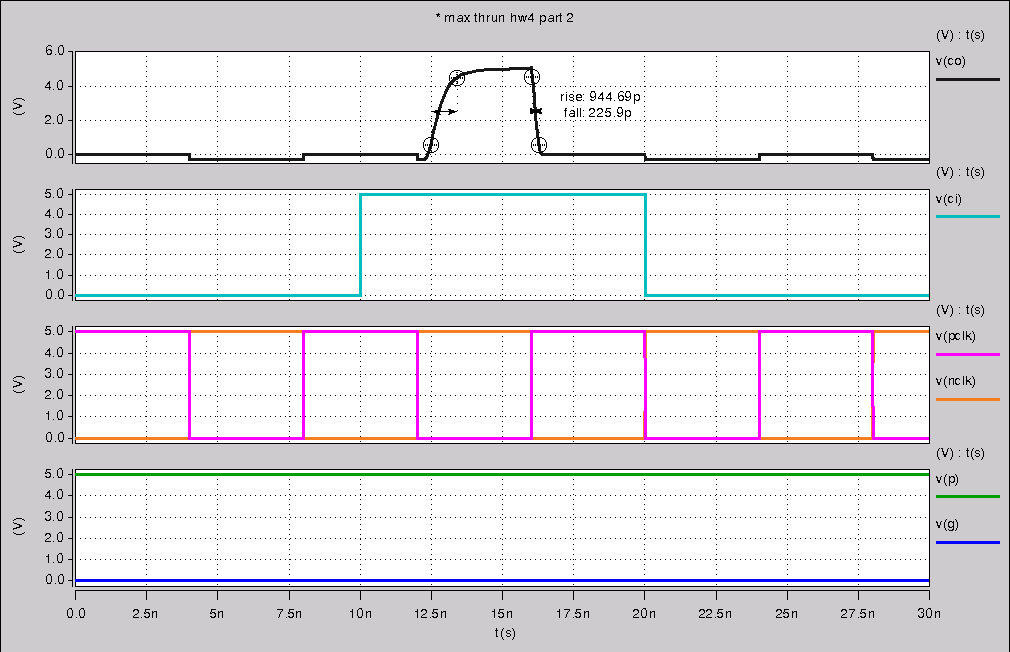
\includegraphics[width=0.8\linewidth]{../part_2.png}
    \caption{Part 2 Simulation Result}
\end{figure}

The clock was then increased until the output only reached 90\% of 5V (4.5V).
The max clock speed was found to be \textbf{380MHz}.

\begin{figure}[H]
    \centering
    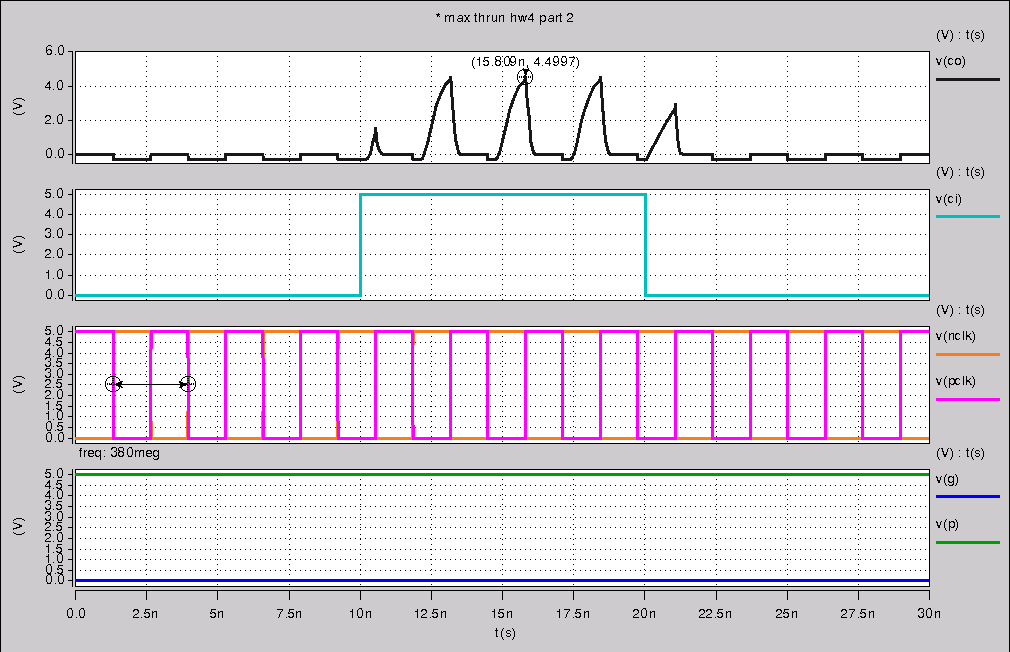
\includegraphics[width=0.8\linewidth]{../part_2_fast.png}
    \caption{Part 2 Simulation Result (Max Clock Speed)}
\end{figure}

\newpage
\section*{Part 3}

Constructing a 4-bit carry chain was achieved by simply instantiating 4 carry
slices and chaining the carries together. The same worst case conditions were
setup for each slice which allows for a pulse at slice 0 to propagate all the
way through the last slice, slice 3.

\lstinputlisting[caption=Part 3 Spice File]{../part_3.sp}

\newpage
The simulation result for the 4-bit configuration is shown below. We can
clearly see the input pulse propagate between each slice with each slice adding
some delay. The total propagation delay was found to be \textbf{3.688ns}. For
this simulation we skipped to directly changing the clock speed until the
amplitude of the last carry out was 90\% of 5V (4.5V). We found the max clock
speed to be \textbf{117MHz}.

\begin{figure}[H]
    \centering
    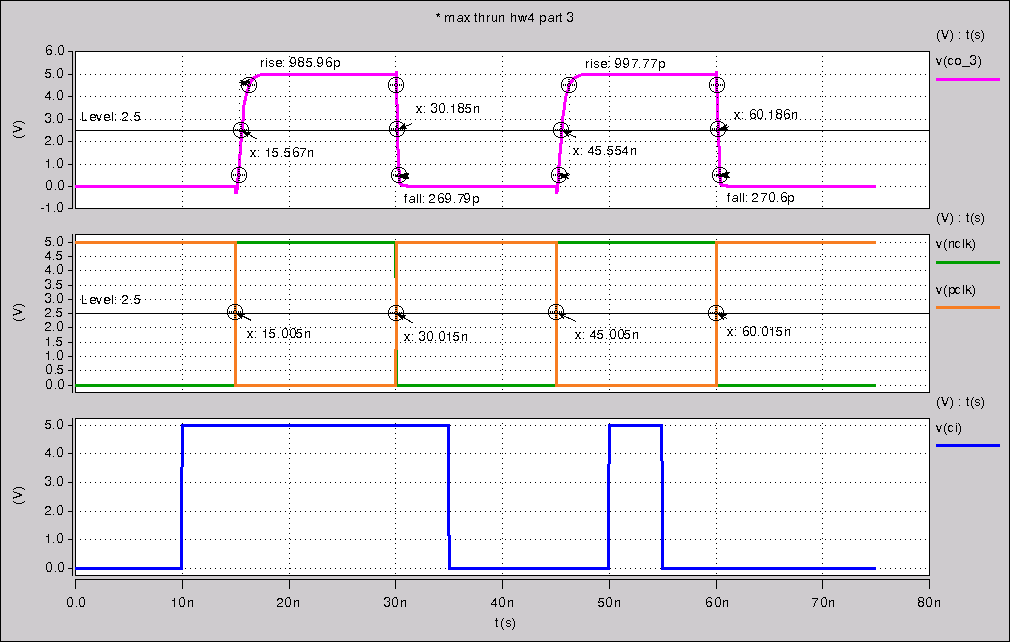
\includegraphics[width=\linewidth]{../part_3.png}
    \caption{Part 3 Simulation Result}
\end{figure}

\newpage
\section*{Part 4}

In order to find the minimum clock speed I first set CI of the first slice to
be constant value of 0V. This should result in the output being flat lined at
0V.  I then decreased the clock speed until I found an interesting glitch
started to become prominent around \textbf{1.75KHz}

\lstinputlisting[caption=Part 4 Spice File]{../part_4.sp}

\newpage
The figure below shows the glitch at 1.7KHz starting to cross 0.5V.

\begin{figure}[H]
    \centering
    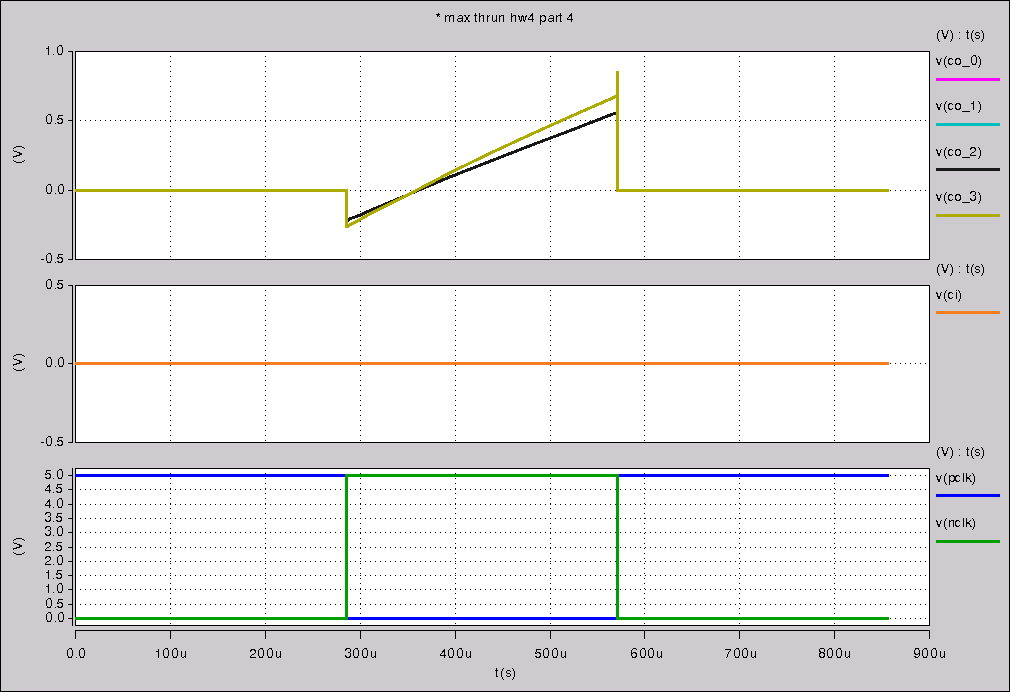
\includegraphics[width=0.8\linewidth]{../part_4.png}
    \caption{Part 4 Simulation Result}
\end{figure}

Decreasing the frequency even further we find that the glitch seems to have
two linear regions and eventually climbs all the way to 5V.

\begin{figure}[H]
    \centering
    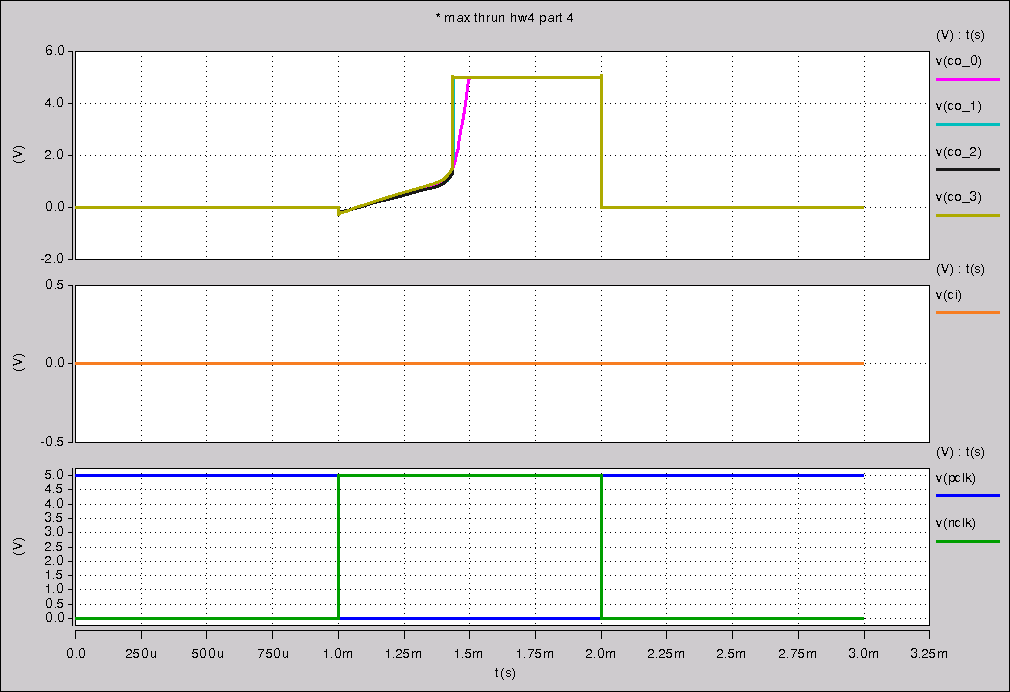
\includegraphics[width=0.8\linewidth]{../part_4_slow.png}
    \caption{Part 4 Simulation Result}
\end{figure}

\newpage
\section*{Final Timing Summary}

\begin{table}[H]
    \centering
    \begin{tabular}{lc}
        \toprule
        \textbf{Component} & \textbf{Max Clock Speed} \\
        \midrule
        P NAND & 530MHz \\
        N NAND & 940MHz \\
   1-Bit Carry & 380MHz \\
   4-Bit Carry & 117MHz \\
        \bottomrule
    \end{tabular}
    \caption{Final Timing Summary}
\end{table}

\section*{What was learned}
This homework provided a great example of designing with dynamic logic. I found
it to be a lot trickier than designing with static logic as you have to ensure
that your clock is running within the small 'working' window. I also found the
results of part 4 really interesting. I did not not initially expect anything
like what I observed. I am still not exactly sure how the carry outputs are
climbing like they are so more time is needed to investigate the root cause.
Overall this homework allowed me to explore a new area of digital design that I
had not previously experienced at all.

\end{document}
